\documentclass[12pt,a4paper]{article}
% \usepackage{ctex}
\usepackage{amsmath,amscd,amsbsy,amssymb,latexsym,url,bm,amsthm}
\usepackage{epsfig,graphicx,subfigure}
\usepackage{enumitem,balance}
\usepackage{wrapfig}
\usepackage{mathrsfs,euscript}
\usepackage[usenames]{xcolor}
\usepackage{hyperref}
\usepackage[vlined,ruled,linesnumbered]{algorithm2e}
\usepackage{array}
\usepackage{tikz}
\hypersetup{colorlinks=true,linkcolor=black}

\newtheorem{theorem}{Theorem}
\newtheorem{lemma}[theorem]{Lemma}
\newtheorem{proposition}[theorem]{Proposition}
\newtheorem{corollary}[theorem]{Corollary}
\newtheorem{exercise}{Exercise}
\newtheorem*{solution}{Solution}
\newtheorem{definition}{Definition}
\theoremstyle{definition}

\renewcommand{\thefootnote}{\fnsymbol{footnote}}

\newcommand{\postscript}[2]
 {\setlength{\epsfxsize}{#2\hsize}
  \centerline{\epsfbox{#1}}}

\renewcommand{\baselinestretch}{1.0}

\setlength{\oddsidemargin}{-0.365in}
\setlength{\evensidemargin}{-0.365in}
\setlength{\topmargin}{-0.3in}
\setlength{\headheight}{0in}
\setlength{\headsep}{0in}
\setlength{\textheight}{10.1in}
\setlength{\textwidth}{7in}
\makeatletter \renewenvironment{proof}[1][Proof] {\par\pushQED{\qed}\normalfont\topsep6\p@\@plus6\p@\relax\trivlist\item[\hskip\labelsep\bfseries#1\@addpunct{.}]\ignorespaces}{\popQED\endtrivlist\@endpefalse} \makeatother
\makeatletter
\renewenvironment{solution}[1][Solution] {\par\pushQED{\qed}\normalfont\topsep6\p@\@plus6\p@\relax\trivlist\item[\hskip\labelsep\bfseries#1\@addpunct{.}]\ignorespaces}{\popQED\endtrivlist\@endpefalse} \makeatother

\begin{document}
\noindent

%========================================================================
\noindent\framebox[\linewidth]{\shortstack[c]{
\Large{\textbf{Lab10-Turing Machine}}\vspace{1mm}\\
CS214-Algorithm and Complexity, Xiaofeng Gao \& Lei Wang, Spring 2021.}}
\begin{center}
\footnotesize{\color{red}$*$ If there is any problem, please contact TA Yihao Xie. }

\footnotesize{\color{blue}$*$ Name: Wendi Chen  \quad Student ID: 519021910071 \quad Email: chenwendi-andy@sjtu.edu.cn}
\end{center}

\begin{enumerate}
    \item Design a one-tape TM $M$ that computes the function $f(x, y) = \lfloor x/y \rfloor$, where $x$ and $y$ are positive integers $(x > y)$. The alphabet is $\{1, 0, \Box, \triangleright, \triangleleft\}$, and the inputs are $x$ "1"s, $\Box$ and $y$ "1"s. Below is the initial configuration for input $x=7$ and $y=3$. The result $z=f(x,y)$ should also be represented in the form of $z$ "1"s on the tape with pattern of $\rhd 111\cdots 111\lhd$, which is $\rhd 11\lhd$ for the example.
    
	\begin{center}
		\begin{tabular}{ll|c|c|c|c|c|c|c|c|c|c|c|c|c|c}
			& \multicolumn{14}{c}{Initial Configuration}\\[5pt]
			\cline{2-16}
			& & $\triangleright$ &  1  & 1 & 1 & 1 & 1 & 1 & 1 & $\Box$ & 1 & 1 & 1 & $ \triangleleft$ & \\
			\cline{2-16}
			\multicolumn{2}{c}{} & \multicolumn{1}{c}{$\uparrow$} & \multicolumn{11}{c}{}\\[-4px]
			\multicolumn{2}{c}{} & \multicolumn{1}{c}{$q_S$} & \multicolumn{11}{c}{}	
		\end{tabular}
	\end{center}

    \begin{enumerate}
	\item
	Please describe your design and then write the specifications of $M$ in the form like $\langle q_S, \triangleright \rangle \rightarrow \langle q_1, \triangleright,  R\rangle$. Explain the transition functions in detail.
	
	\item
	Please draw the state transition diagram.
	
	\item
	Show briefly and clearly the whole process from initial to final configurations for input $x = 7$ and $y = 3$. You may start like this:
	$$(q_s,\underline{\triangleright}  1  1  1  1  1  1  1  \Box 1  1  1   \triangleleft)
	\vdash (q_1,\triangleright  \underline{1}  1  1  1  1  1  1  \Box 1  1  1   \triangleleft)
	\vdash^* (q_1,\triangleright  1  1  1  1  1  1  1  \underline{\Box} 1  1  1   \triangleleft)
	\vdash (q_2,\triangleright  1  1  1  1  1  1  1  \Box \underline{1}  1  1   \triangleleft)$$
	
	\par{\color{blue}(Note that for simplicity, we write $(q_1,\triangleright  \underline{1}  1  1  1  1  1  1  \Box 1  1  1   \triangleleft)\vdash^* (q_1,\triangleright  1  1  1  1  1  1  1  \underline{\Box} 1  1  1   \triangleleft)$ if the corresponding transaction repeats on multiple inputs with the same state.)}
	
\end{enumerate}
    
    \begin{solution}
    ~
    \begin{enumerate}
        \item 
        Let us show the \textbf{basic idea} first. Generally, we want to compare the symbols on the both sides of the``splitting $\Box$" and use ``0" to denote the symbol that has been compared.  And after one iteration, the tape become
        \begin{center}
		\begin{tabular}{ll|c|c|c|c|c|c|c|c|c|c|c|c|c|c}
			\cline{2-16}
			& & $\triangleright$ &  1  & 1 & 1 & 1 & 0 & 0 & 0 & $\Box$ & 0 & 0 & 0 & $ \triangleleft$ & \\
			\cline{2-16}
		\end{tabular}
	    \end{center}
	    Then, we go to the every left of the tape and change the first symbol which is not ``$\Box$" or ``$\triangleright$" to ``$\Box$", which represents a counter. 
	    \begin{center}
		\begin{tabular}{ll|c|c|c|c|c|c|c|c|c|c|c|c|c|c}
			\cline{2-16}
			& & $\triangleright$ &  $\Box$  & 1 & 1 & 1 & 0 & 0 & 0 & $\Box$ & 0 & 0 & 0 & $ \triangleleft$ & \\
			\cline{2-16}
		\end{tabular}
	    \end{center}
	    Next, we update the tape so that we can do the next iteration. Remember that we need to compensate one ``1".
	    \begin{center}
		\begin{tabular}{ll|c|c|c|c|c|c|c|c|c|c|c|c|c|c}
			\cline{2-16}
			& & $\triangleright$ &  $\Box$  & 1 & 1 & 1 & 1 & $\Box$ & 1 & 1 & 1  & $\triangleleft$ & 0 & $ \triangleleft$ & \\
			\cline{2-16}
		\end{tabular}
	    \end{center}
	    After that, we can finish the next iteration.
	    \begin{center}
		\begin{tabular}{ll|c|c|c|c|c|c|c|c|c|c|c|c|c|c}
			\cline{2-16}
			& & $\triangleright$ &  $\Box$  & $\Box$ & 1 & $\Box$ & 1 & 1 & 1 & $\triangleleft$ & 0  & $\triangleleft$ & 0 & $ \triangleleft$ & \\
			\cline{2-16}
		\end{tabular}
	    \end{center}
	    And when we do the third iteration, there is no enough symbol on the left for comparison.
	    \begin{center}
		\begin{tabular}{ll|c|c|c|c|c|c|c|c|c|c|c|c|c|c}
			\cline{2-16}
			& & $\triangleright$ &  $\Box$  & $\Box$ & 0 & $\Box$ & 0 & 0 & 1 & $\triangleleft$ & 0  & $\triangleleft$ & 0 & $ \triangleleft$ & \\
			\cline{2-16}
		\end{tabular}
	    \end{center}
	    So we can do the finishing steps: change the first ``0" or the ``splitting $\Box$" to ``$ \triangleleft$" and replace other ``$\Box$" on the left with ``1".
	    \begin{center}
		\begin{tabular}{ll|c|c|c|c|c|c|c|c|c|c|c|c|c|c}
			\cline{2-16}
			& & $\triangleright$ &  1  & 1 & $\triangleleft$ & $\Box$ & 0 & 0 & 1 & $\triangleleft$ & 0  & $\triangleleft$ & 0 & $ \triangleleft$ & \\
			\cline{2-16}
		\end{tabular}
	    \end{center}
	    Here we get the final result.\\
	    ~\\
	    Next, we'll divide the whole process into several parts and try to write the specifications of $M$.\\
	    In part one, we want to do some preparations for the comparison. We need skip the first few ``$\Box$" and move the the right of the ``splitting $\Box$". After we change the state to $q_3$, we're ready to do the comparison.
	    \begin{align*}
	    \langle q_S, \triangleright \rangle \rightarrow \langle q_1, \triangleright,  R\rangle
	    \quad
	    \langle q_1, \Box \rangle \rightarrow \langle q_1, \Box,  R\rangle
	    \quad
	    \langle q_1, 1 \rangle \rightarrow \langle q_2, 1,  R\rangle\\
	    \langle q_2, 1 \rangle \rightarrow \langle q_2, 1,  R\rangle
	    \quad
	    \langle q_2, \Box \rangle \rightarrow \langle q_3, \Box,  R\rangle
	    \end{align*}
	    In part two, we want to do the comparison. Here, we use several states to represents the direction that the head is moving. And we also need to distinguish whether we are now on the left or the right side of the ``splitting $\Box$". 
	    \begin{align*}
	        \langle q_3, 0 \rangle \rightarrow \langle q_3, 0,  R\rangle
	        \quad
	        \langle q_3, 1 \rangle \rightarrow \langle q_4, 0,  L\rangle
	        \quad
	        \langle q_4, 0 \rangle \rightarrow \langle q_4, 0,  L\rangle\\
	        \langle q_4, \Box \rangle \rightarrow \langle q_5, \Box,  L\rangle
	        \quad
	        \langle q_5, 0 \rangle \rightarrow \langle q_5, 0,  L\rangle
	        \quad
	        \langle q_5, 1 \rangle \rightarrow \langle q_6, 0,  R\rangle\\
	        \langle q_6, 0 \rangle \rightarrow \langle q_6, 0,  R\rangle
	        \quad
	        \langle q_6, \Box \rangle \rightarrow \langle q_3, \Box,  R\rangle
	    \end{align*}
	    In part three, we need to update the tape after finishing one iteration. There are many details here, but we don't have to worry. All we need to remember is to move to the every left first and use ``$\Box$" as a counter. Then maintain the number of 1's in the string through a series of operations and try to revert to a pattern similar to the initial tape.
	    \begin{align*}
	        \langle q_3, \triangleleft \rangle \rightarrow \langle q_7, \triangleleft,  L\rangle
	        \quad
	        \langle q_7, 0 \rangle \rightarrow \langle q_7, 0,  L\rangle
	        \quad
	        \langle q_7, \Box \rangle \rightarrow \langle q_8, \Box,  L\rangle\\
	        \langle q_8, 0 \rangle \rightarrow \langle q_8, 0,  L\rangle
	        \quad
	        \langle q_8, 1 \rangle \rightarrow \langle q_8, 1,  L\rangle
	        \\
	        \langle q_8, \triangleright \rangle \rightarrow \langle q_9, \triangleright,  R\rangle
	        \quad
	        \langle q_8, \Box \rangle \rightarrow \langle q_9, \Box,  R\rangle\\
	        \langle q_9, 1 \rangle \rightarrow \langle q_{10}, \Box,  R\rangle
	        \quad
	        \langle q_{10}, 1 \rangle \rightarrow \langle q_{10}, 1,  R\rangle
	        \quad
	        \langle q_{10}, 0 \rangle \rightarrow \langle q_{11}, 1,  R\rangle\\
	        \langle q_{11}, 0 \rangle \rightarrow \langle q_{12}, \Box,  R\rangle
	        \quad
	        \langle q_{12}, 0 \rangle \rightarrow \langle q_{12}, 1,  R\rangle
	        \quad
	        \langle q_{12}, \Box \rangle \rightarrow \langle q_{13}, 1,  R\rangle\\
	        \langle q_{9}, 0 \rangle \rightarrow \langle q_{10}, \Box,  R\rangle
	        \quad
	        \langle q_{11}, \Box \rangle \rightarrow \langle q_{12}, \Box,  R\rangle
	        \quad 
	        \langle q_{12}, \triangleleft \rangle \rightarrow \langle q_{15}, \triangleleft,  L\rangle
	        \\
	        \langle q_{13}, 0 \rangle \rightarrow \langle q_{14}, 1,  R\rangle
	        \quad
	        \langle q_{14}, 0\rangle \rightarrow \langle q_{15}, \triangleleft,  L\rangle
	        \quad
	        \langle q_{15}, \Box\rangle \rightarrow \langle q_{15},\Box,  L\rangle\\
	        \langle q_{15}, 1\rangle \rightarrow \langle q_{15},1,  L\rangle
	        \quad
	        \langle q_{15}, \triangleright\rangle \rightarrow \langle q_{1},\triangleright,  R\rangle
	    \end{align*}
	    At last, let us do the finishing steps. We change ``$\Box$" to ``1" to represent the result and mark the ``$\triangleleft$".
	    \begin{align*}
	        \langle q_5, \Box\rangle \rightarrow \langle q_{16},\Box,  R\rangle
	        \quad
	        \langle q_{16}, 0\rangle \rightarrow \langle q_{17},\triangleleft,  L\rangle
	        \quad
	        \langle q_{16}, \Box\rangle \rightarrow \langle q_{17},\triangleleft,  L\rangle\\
	         \langle q_{10}, \Box \rangle \rightarrow \langle q_{17}, \triangleleft,  L\rangle
	        \quad
	        \langle q_{17}, \Box\rangle \rightarrow \langle q_{17},1,  L\rangle
	        \quad
	         \langle q_{17},  \triangleright\rangle \rightarrow \langle q_{H},\triangleright,  S\rangle
	    \end{align*}
	    \newpage
	    \item
	    Here is the state transition diagram.
	    
	\begin{center}
    \begin{tikzpicture}[scale=0.18]
    \tikzstyle{every node}+=[inner sep=0pt]
    \draw [black] (9.5,-3.5) circle (2.2);
    \draw (9.5,-3.5) node {$q_s$};
    \draw [black] (9.5,-14) circle (2.2);
    \draw (9.5,-14) node {$q_1$};
    \draw [black] (34.2,-7.3) circle (2.2);
    \draw (34.2,-7.3) node {$q_2$};
    \draw [black] (49.1,-7.3) circle (2.2);
    \draw (49.1,-7.3) node {$q_3$};
    \draw [black] (63.1,-7.3) circle (2.2);
    \draw (63.1,-7.3) node {$q_4$};
    \draw [black] (77.1,-21.6) circle (2.2);
    \draw (77.1,-21.6) node {$q_5$};
    \draw [black] (65.6,-21.6) circle (2.2);
    \draw (65.6,-21.6) node {$q_6$};
    \draw [black] (52.8,-21.6) circle (2.2);
    \draw (52.8,-21.6) node {$q_7$};
    \draw [black] (37.5,-21.6) circle (2.2);
    \draw (37.5,-21.6) node {$q_8$};
    \draw [black] (14.8,-21.6) circle (2.2);
    \draw (14.8,-21.6) node {$q_9$};
    \draw [black] (45,-43.9) circle (2.2);
    \draw (45,-43.9) node {$q_{10}$};
    \draw [black] (37.5,-53.5) circle (2.2);
    \draw (37.5,-53.5) node {$q_{11}$};
    \draw [black] (23.6,-42.4) circle (2.2);
    \draw (23.6,-42.4) node {$q_{12}$};
    \draw [black] (14.2,-49.4) circle (2.2);
    \draw (14.2,-49.4) node {$q_{13}$};
    \draw [black] (9.5,-32.4) circle (2.2);
    \draw (9.5,-32.4) node {$q_{15}$};
    \draw [black] (4.3,-49.4) circle (2.2);
    \draw (4.3,-49.4) node {$q_{14}$};
    \draw [black] (73.1,-34.6) circle (2.2);
    \draw (73.1,-34.6) node {$q_{16}$};
    \draw [black] (62.2,-43.9) circle (2.2);
    \draw (62.2,-43.9) node {$q_{17}$};
    \draw [black] (73.1,-53.5) circle (2.2);
    \draw (73.1,-53.5) node {$q_{H}$};
    \draw [black] (73.1,-53.5) circle (1.6);
    
    \draw [black] (9.5,-5.7) -- (9.5,-11.8);
    \fill [black] (9.5,-11.8) -- (10,-11) -- (9,-11);
    \draw (9,-8.75) node [left] {$\triangleright/\triangleright,R$};
    \draw [black] (8.018,-15.615) arc (-14.81106:-302.81106:1.65);
    \draw (4.13,-16.64) node [left] {$\Box/\Box,R$};
    \fill [black] (7.32,-13.81) -- (6.67,-13.12) -- (6.42,-14.08);
    \draw [black] (11.62,-13.42) -- (32.08,-7.88);
    \fill [black] (32.08,-7.88) -- (31.17,-7.6) -- (31.44,-8.57);
    \draw (24.17,-11.33) node [below] {$1/1,R$};
    \draw [black] (33.23,-5.335) arc (234:-54:1.65);
    \draw (34.2,-1.85) node [above] {$1/1,R$};
    \fill [black] (35.17,-5.33) -- (36.04,-4.98) -- (35.24,-4.39);
    \draw [black] (36.4,-7.3) -- (46.9,-7.3);
    \fill [black] (46.9,-7.3) -- (46.1,-6.8) -- (46.1,-7.8);
    \draw (41.65,-7.8) node [below] {$\Box/\Box,R$};
    \draw [black] (48.13,-5.335) arc (234:-54:1.65);
    \draw (49.1,-1.85) node [above] {$0/0,R$};
    \fill [black] (50.07,-5.33) -- (50.94,-4.98) -- (50.14,-4.39);
    \draw [black] (51.3,-7.3) -- (60.9,-7.3);
    \fill [black] (60.9,-7.3) -- (60.1,-6.8) -- (60.1,-7.8);
    \draw (56.1,-7.8) node [below] {$1/0,L$};
    \draw [black] (62.995,-5.111) arc (210.47402:-77.52598:1.65);
    \draw (68,-2.23) node [above] {$0/0,L$};
    \fill [black] (64.77,-5.89) -- (65.72,-5.91) -- (65.21,-5.05);
    \draw [black] (64.99,-8.425) arc (57.43493:31.35037:34.918);
    \fill [black] (76.02,-19.69) -- (76.03,-18.74) -- (75.17,-19.26);
    \draw (71.67,-11.95) node [right] {$\Box/\Box,L$};
    \draw [black] (78.7,-23.098) arc (74.6193:-213.3807:1.65);
    \draw (81.66,-26.8) node [below] {$0/0,L$};
    \fill [black] (76.88,-23.78) -- (76.19,-24.42) -- (77.15,-24.68);
    \draw [black] (74.9,-21.6) -- (67.8,-21.6);
    \fill [black] (67.8,-21.6) -- (68.6,-22.1) -- (68.6,-21.1);
    \draw (71.35,-21.1) node [above] {$1/0,R$};
\draw [black] (64.222,-23.304) arc (-11.24572:-299.24572:1.65);
\draw (60.39,-24.7) node [left] {$0/0,R$};
\fill [black] (63.41,-21.54) -- (62.72,-20.9) -- (62.53,-21.88);
    \draw [black] (63.94,-20.16) -- (50.76,-8.74);
    \fill [black] (50.76,-8.74) -- (51.04,-9.64) -- (51.69,-8.89);
    \draw (63.36,-13.96) node [above] {$\Box/\Box,R$};
    \draw [black] (49.65,-9.43) -- (52.25,-19.47);
    \fill [black] (52.25,-19.47) -- (52.53,-18.57) -- (51.56,-18.82);
    \draw (50.19,-14.93) node [left] {$\triangleleft/\triangleleft,L$};
    \draw [black] (53.77,-23.565) arc (54:-234:1.65);
    \draw (52.8,-27.05) node [below] {$0/0,L$};
    \fill [black] (51.83,-23.57) -- (50.96,-23.92) -- (51.76,-24.51);
    \draw [black] (50.6,-21.6) -- (39.7,-21.6);
    \fill [black] (39.7,-21.6) -- (40.5,-22.1) -- (40.5,-21.1);
    \draw (45.15,-21.1) node [above] {$\Box/\Box,L$};
    \draw [black] (36.53,-19.635) arc (234:-54:1.65);
    \draw (37.5,-16.15) node [above] {$0/0,L$};
    \fill [black] (38.47,-19.63) -- (39.34,-19.28) -- (38.54,-18.69);
    \draw [black] (39.312,-22.832) arc (83.52872:-204.47128:1.65);
    \draw (42.93,-26.41) node [below] {$1/1,L$};
    \fill [black] (37.62,-23.79) -- (37.04,-24.53) -- (38.03,-24.64);


    \draw [black] (16.798,-20.682) arc (112.14169:67.85831:24.812);
    \fill [black] (16.8,-20.68) -- (17.73,-20.84) -- (17.35,-19.92);
    \draw (26.15,-18.35) node [above] {$\Box/\Box,R$};
    \draw [black] (43.023,-42.936) arc (-116.64169:-136.24341:97.56);
    \fill [black] (43.02,-42.94) -- (42.53,-42.13) -- (42.08,-43.02);
    \draw (24.31,-34.71) node [below] {$1/\Box,R$};
    \draw [black] (45.154,-41.714) arc (203.69336:-84.30664:1.65);
    \draw (50.49,-39.12) node [above] {$1/1,R$};
    \fill [black] (46.83,-42.69) -- (47.76,-42.83) -- (47.36,-41.91);
    \draw [black] (44.494,-46.038) arc (-18.46184:-57.53563:12.245);
    \fill [black] (39.45,-52.49) -- (40.4,-52.48) -- (39.86,-51.64);
    \draw (43.1,-51.11) node [right] {$0/1,R$};
    \draw [black] (25.644,-43.212) arc (65.98954:36.79145:26.939);
    \fill [black] (25.64,-43.21) -- (26.17,-43.99) -- (26.58,-43.08);
    \draw (36,-46.27) node [above] {$0/\Box,R$};
    \draw [black] (25.174,-40.876) arc (161.80408:-126.19592:1.65);
    \draw (29.08,-40.22) node [right] {$0/1,R$};
    \fill [black] (25.77,-42.72) -- (26.37,-43.45) -- (26.68,-42.5);
    \draw [black] (21.84,-43.71) -- (15.96,-48.09);
    \fill [black] (15.96,-48.09) -- (16.9,-48.01) -- (16.31,-47.21);
    \draw (14.4,-45.4) node [above] {$\Box/1,R$};
    \draw [black] (16.721,-22.672) arc (60.39067:46.72422:139.421);
    \fill [black] (43.41,-42.38) -- (43.17,-41.47) -- (42.49,-42.19);
    \draw (35.16,-31.23) node [above] {$0/\Box,R$};
    \draw [black] (35.819,-54.911) arc (-57.06751:-200.1515:8.92);
    \fill [black] (22.6,-44.35) -- (21.85,-44.93) -- (22.79,-45.27);
    \draw (19.4,-54.89) node [below] {$\Box/\Box,R$};
    \draw [black] (21.81,-41.13) -- (11.29,-33.67);
    \fill [black] (11.29,-33.67) -- (11.66,-34.54) -- (12.24,-33.73);
    \draw (10.05,-37.9) node [below] {$\triangleleft/\triangleleft,L$};
    \draw [black] (12,-49.4) -- (6.5,-49.4);
    \fill [black] (6.5,-49.4) -- (7.3,-49.9) -- (7.3,-48.9);
    \draw (9.25,-48.9) node [above] {$0/1,R$};
    \draw [black] (4.192,-47.203) arc (-179.89816:-214.11774:23.181);
    \fill [black] (8.18,-34.16) -- (7.32,-34.54) -- (8.15,-35.1);
    \draw (4.44,-39.76) node [left] {$0/\triangleleft,L$};
    \draw [black] (7.372,-31.877) arc (283.92677:-4.07323:1.65);
    \draw (5.16,-27.77) node [left] {$\Box/\Box,L$};
    \fill [black] (8.62,-30.39) -- (8.91,-29.5) -- (7.94,-29.74);
    \draw [black] (10.25,-30.341) arc (187.70544:-100.29456:1.65);
    \draw (13.61,-27.51) node [right] {$1/1,L$};
    \fill [black] (11.59,-31.74) -- (12.45,-32.13) -- (12.32,-31.14);
    \draw [black] (9.5,-30.2) -- (9.5,-16.2);
    \fill [black] (9.5,-16.2) -- (9,-17) -- (10,-17);
    \draw (9,-23.2) node [left] {$\triangleright/\triangleright,R$};
    \draw [black] (73.36,-32.416) arc (171.23323:154.56131:31.982);
    \fill [black] (73.36,-32.42) -- (73.98,-31.7) -- (72.99,-31.55);
    \draw (73.63,-27.26) node [left] {$\Box/\Box,R$};
    \draw [black] (62.654,-41.752) arc (162.00046:98.94189:10.373);
    \fill [black] (62.65,-41.75) -- (63.38,-41.15) -- (62.43,-40.84);
    \draw (60.78,-36.57) node [above] {$0/\triangleleft,L$};
    \draw [black] (71.43,-36.03) -- (63.87,-42.47);
    \fill [black] (63.87,-42.47) -- (64.81,-42.33) -- (64.16,-41.57);
    \draw (74.16,-39.74) node [below] {$\Box/\triangleleft,L$};
    \draw [black] (47.2,-43.9) -- (60,-43.9);
    \fill [black] (60,-43.9) -- (59.2,-43.4) -- (59.2,-44.4);
    \draw (53.6,-44.4) node [below] {$\Box/\triangleleft,L$};
    \draw [black] (62.851,-45.992) arc (45.02737:-242.97263:1.65);
    \draw (59.61,-49.71) node [below] {$\Box/1,L$};
    \fill [black] (60.94,-45.69) -- (60.02,-45.9) -- (60.72,-46.61);
    \draw [black] (63.85,-45.35) -- (71.45,-52.05);
    \fill [black] (71.45,-52.05) -- (71.18,-51.14) -- (70.52,-51.89);
    \draw (75.66,-48.21) node [above] {$\triangleright/\triangleright,S$};
    \draw [black] (35.31,-21.81) arc (-85.11799:-94.88201:107.633);
\fill [black] (16.99,-21.81) -- (17.74,-22.38) -- (17.83,-21.38);
\draw (26.15,-22.7) node [below] {$\triangleright/\triangleright,R$};
    \end{tikzpicture}
    \end{center}
    
    \item
    In this section, we'll show the whole process. For simplicity, we only retain the symbols that is between the first ``$\triangleright$" and the corresponding ``$\triangleleft$".
    \begin{align*}
     (q_s,\underline{\triangleright}  1  1  1  1  1  1  1  \Box 1  1  1   \triangleleft)
	\vdash (q_1,\triangleright  \underline{1}  1  1  1  1  1  1  \Box 1  1  1   \triangleleft)
	\vdash (q_2,\triangleright  1  \underline{1}  1  1  1  1  1  \Box 1  1  1   \triangleleft)
	\vdash^{*} (q_2,\triangleright  1  1  1  1  1  1  1  \underline{\Box} 1  1  1   \triangleleft)\\
	\vdash (q_3,\triangleright  1  1  1  1  1  1  1  \Box \underline{1}  1  1   \triangleleft)
	\vdash (q_4,\triangleright  1  1  1  1  1  1  1  \underline{\Box} 0  1  1   \triangleleft)
	\vdash (q_5,\triangleright  1  1  1  1  1  1  \underline{1}  \Box 0  1  1   \triangleleft)
	\vdash (q_6,\triangleright  1  1  1  1  1  1  0  \underline{\Box} 0  1  1   \triangleleft)\\
	\vdash (q_3,\triangleright  1  1  1  1  1  1  0  \Box \underline{0}  1  1   \triangleleft)
	\vdash (q_3,\triangleright  1  1  1  1  1  1  0  \Box 0  \underline{1}  1   \triangleleft)
    \end{align*}
    Next few steps follow the same pattern, so we omit it.
    \begin{align*}
     (q_5,\triangleright  1  1  1  1  \underline{1}  0  0  \Box 0  0  0   \triangleleft)
     \vdash (q_6,\triangleright  1  1  1  1  0  \underline{0}  0  \Box 0  0  0   \triangleleft)
     \vdash^{*}(q_6,\triangleright  1  1  1  1  0  0  0  \underline{\Box} 0  0  0   \triangleleft)\\
     \vdash(q_3,\triangleright  1  1  1  1  0  0  0  \Box \underline{0}  0  0   \triangleleft)
     \vdash^{*}(q_3,\triangleright  1  1  1  1  0  0  0  \Box 0  0  0   \underline{\triangleleft})
     \vdash(q_7,\triangleright  1  1  1  1  0  0  0  \Box 0  0  \underline{0}   \triangleleft)\\
     \vdash^{*}(q_7,\triangleright  1  1  1  1  0  0  0  \underline{\Box} 0  0  0   \triangleleft)
     \vdash(q_8,\triangleright  1  1  1  1  0  0  \underline{0}  \Box 0  0  0   \triangleleft)
     \vdash^{*}(q_8,\underline{\triangleright}  1  1  1  1  0  0  0  \Box 0  0  0   \triangleleft)\\
     \vdash(q_9,\triangleright  \underline{1}  1  1  1  0  0  0  \Box 0  0  0   \triangleleft)
     \vdash(q_{10},\triangleright  \Box  \underline{1}  1  1  0  0  0  \Box 0  0  0   \triangleleft)
     \vdash^{*}(q_{10},\triangleright  \Box  1  1  1  \underline{0}  0  0  \Box 0  0  0   \triangleleft)\\
     \vdash(q_{11},\triangleright  \Box  1  1  1  1  \underline{0}  0  \Box 0  0  0   \triangleleft)
     \vdash(q_{12},\triangleright  \Box  1  1  1  1  \Box  \underline{0}  \Box 0  0  0   \triangleleft)
     \vdash(q_{12},\triangleright  \Box  1  1  1  1  \Box  1  \underline{\Box} 0  0  0   \triangleleft)\\
     \vdash(q_{13},\triangleright  \Box  1  1  1  1  \Box  1  1  \underline{0}  0  0   \triangleleft)
     \vdash(q_{14},\triangleright  \Box  1  1  1  1  \Box  1  1  1  \underline{0}  0   \triangleleft)
     \vdash(q_{15},\triangleright  \Box  1  1  1  1  \Box  1  1  \underline{1}  \triangleleft)\\
     \vdash^{*}(q_{15},\underline{\triangleright}  \Box  1  1  1  1  \Box  1  1  1  \triangleleft)
     \vdash(q_{1},\triangleright  \underline{\Box}  1  1  1  1  \Box  1  1  1  \triangleleft)
    \end{align*}
    Next several steps follow the above pattern and we omit it.
    \begin{align*}
        (q_{3},\triangleright  \Box  \Box  0 \Box  0 \underline{1}  1  \triangleleft)
        \vdash
        (q_{4},\triangleright  \Box  \Box  0 \Box  \underline{0} 0  1  \triangleleft)
        \vdash
        (q_{4},\triangleright  \Box  \Box  0 \underline{\Box}  0 0  1  \triangleleft)\\
        \vdash
        (q_{5},\triangleright  \Box  \Box  \underline{0} \Box  0 0  1  \triangleleft)
        \vdash
        (q_{5},\triangleright  \Box  \underline{\Box}  0 \Box  0 0  1  \triangleleft)
        \vdash
        (q_{16},\triangleright  \Box  \Box  \underline{0} \Box  0 0  1  \triangleleft)\\
        \vdash
        (q_{17},\triangleright  \Box  \underline{\Box}  \triangleleft )
        \vdash
        (q_{17},\triangleright  \underline{\Box}  1  \triangleleft )
        \vdash
        (q_{17},\underline{\triangleright}  1  1  \triangleleft )
        \vdash
        (q_{H},\underline{\triangleright}  1  1  \triangleleft )
    \end{align*}
    In addition, I also write a program (you can refer to \emph{Code-TM-Program.txt}) and test it through a simulator (\emph{https://alistat.eu/online/turingmachinesimulator}). Here 2 stands for $\triangleright$, 3 stands for $\triangleleft$ and 4 stands for $\Box$. You can see our design returns the right answer (Figure \ref{Fig-TM}).
    
    \begin{figure}[!htbp]
    	\centering
    	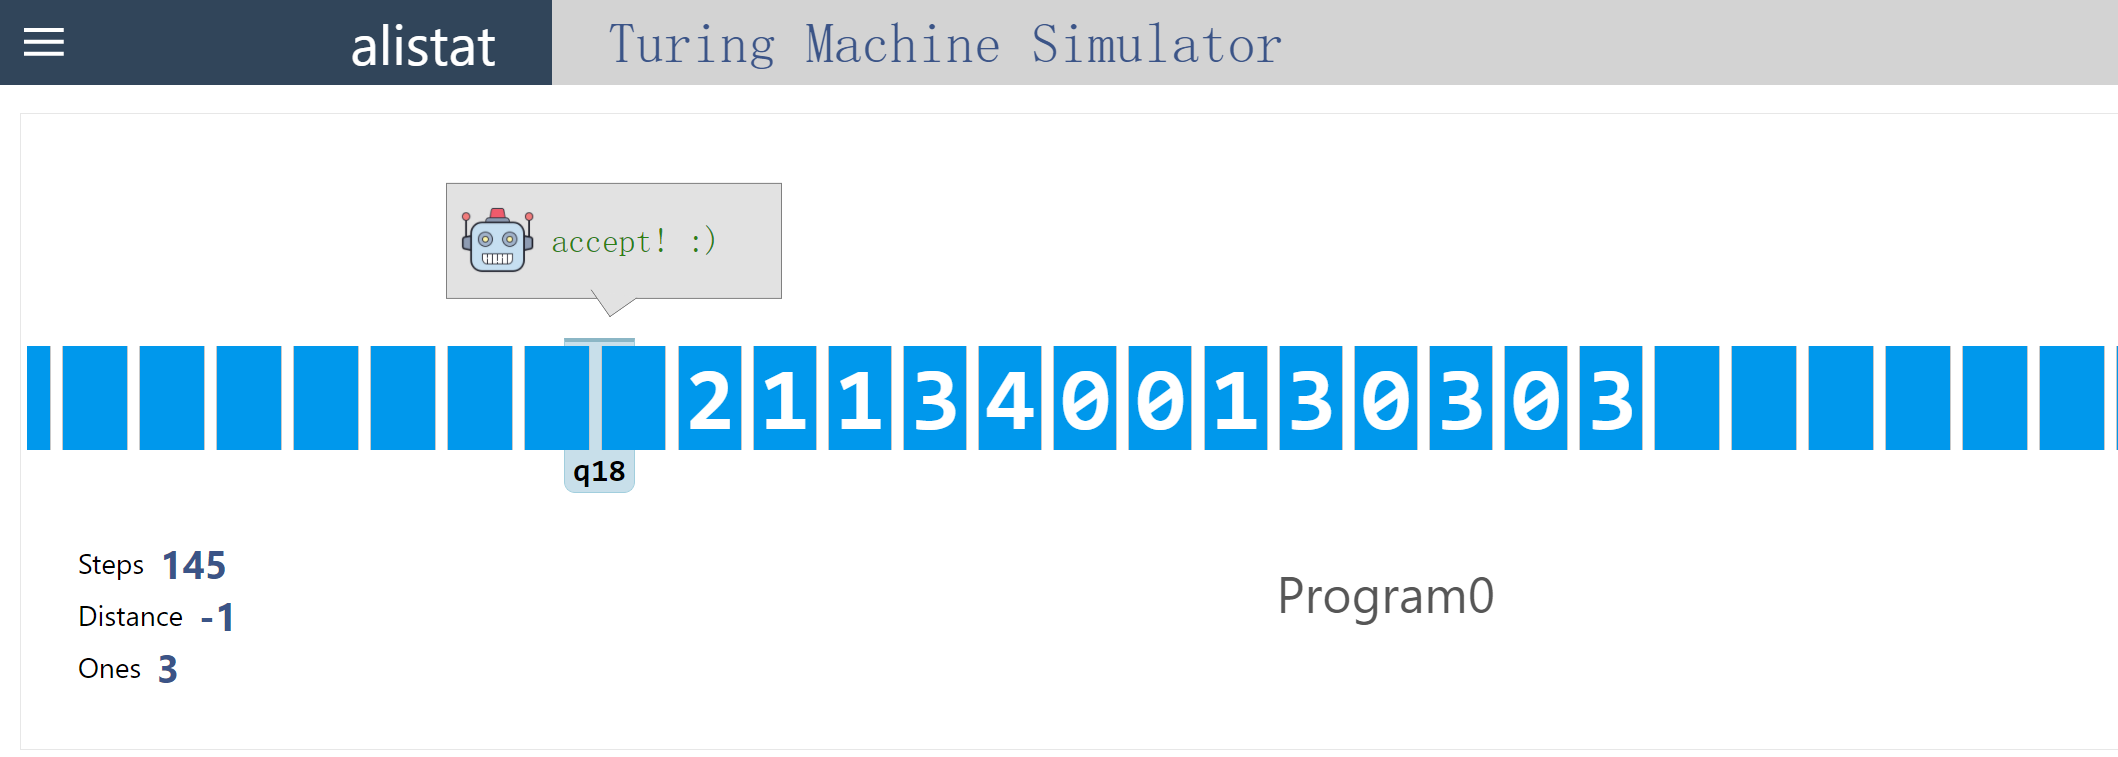
\includegraphics[width=0.7\textwidth]{Fig-TM.png}
    	\caption{Using the Simulator to Check the Design}
    	\label{Fig-TM}
    \end{figure}
    \end{enumerate}
    \end{solution}
    \newpage
    \item 
    Given the alphabet $\{1, 0, \Box, \triangleright, \triangleleft\}$, design a time efficient 3-tape TM $M$ to compute $f:\{0,1\}^*\rightarrow\{0,1\}$ which verifies whether the number of 0 and the number of 1 are the same in an input consisting of only 0's and 1's. $M$ should output 1 if the numbers are the same, and 0 otherwise. For eample, for the input tape $\triangleright 001101\triangleleft$, $M$ should output 1
    
    \begin{enumerate}
	    \item
	    Please describe your design and then write the specifications of $M$ in the form like $\langle q_S, \triangleright, \triangleright, \triangleright \rangle \rightarrow \langle q_1, \triangleright,\triangleright,  R, R, S \rangle$. Explain the transition functions in detail.
	    
	    \item 
	    Show the time complexity for one-tape TM $M'$ to compute the same function $f$ with $n$ symbols in the input and give a brief description of such $M'$ .
	
	\end{enumerate}
	
	\begin{solution}
	~
	\begin{enumerate}
	    \item
	    Initially the input string is located on the first tape like ``$\triangleright001101\triangleleft\Box\Box\cdots$", strings on all other tapes are  ``$\triangleright\Box\Box\cdots$". The idea is to copy the ``1"s on the first tape to the second tape and then compare the number of ``1"s on the second tape with the number of ``0"s on the first tape. Thus, let us write the specifications of M.\\
	    \textbf{Start State:} In this stage, we do some preparations for copying.
	    \begin{align*}
	        \langle q_S, \triangleright, \triangleright, \triangleright \rangle \rightarrow \langle q_C, \triangleright,\triangleright,  R, R, R \rangle
	    \end{align*}
	    \textbf{Begin to copy:} When copying, we just copy ``1''s to the second tape. Therefore, we skip those ``0"s. When arriving at the every right of the input tape, we finish this stage.
	    \begin{align*}
	        \langle q_C, 0, \Box, \Box \rangle \rightarrow \langle q_C, \Box,\Box,  R, S , S \rangle\\
	        \langle q_C, 1, \Box, \Box \rangle \rightarrow \langle q_C, 1,\Box,  R, R , S \rangle\\
	        \langle q_C, \triangleleft, \Box, \Box \rangle \rightarrow \langle q_l, \Box,\Box,  L, S , S \rangle
	    \end{align*}
	    \textbf{Return back to the leftmost:} This stage is quite trivial. We just move the head of the input tape to the every left of it.
	    \begin{align*}
	        \langle q_l, 0, \Box, \Box \rangle \rightarrow \langle q_l, \Box,\Box,  L, S , S \rangle\\
	        \langle q_l, 1, \Box, \Box \rangle \rightarrow \langle q_l, \Box,\Box,  L, S , S \rangle\\
	        \langle q_l, \triangleright, \Box, \Box \rangle \rightarrow \langle q_t, \Box,\Box,  R, L , S \rangle
	    \end{align*}
	    \textbf{Begin to compare:} When doing the comparison, we want to match one ``1" on the second tape with one ``0" on the input tape. We should be careful to determine when we should change the state. There're three cases and we can solve them one by one.
	    \begin{align*}
	        \langle q_t, 0, 1, \Box \rangle \rightarrow \langle q_t, 1,\Box,  R, L , S \rangle\\
	        \langle q_t, 1, 1, \Box \rangle \rightarrow \langle q_t, 1,\Box,  R, S , S \rangle\\
	        \langle q_t, 1, \triangleright, \Box \rangle \rightarrow \langle q_t, \triangleright,\Box,  R, S , S \rangle\\
	        \langle q_t, \triangleleft, \triangleright, \Box \rangle \rightarrow \langle q_r, \triangleright,1,  S, S , R
	        \rangle\\
	        \langle q_t, 0, \triangleright, \Box \rangle \rightarrow \langle q_r, \triangleright,0,  S, S , R\rangle\\
	        \langle q_t, \triangleleft, 1, \Box \rangle \rightarrow \langle q_r, 1,0,  S, S , R
	        \rangle
	    \end{align*}
	    \textbf{Ready to terminate:} There're also three cases accordingly.
	    \begin{align*}
	        \langle q_r, \triangleleft, \triangleright, \Box \rangle \rightarrow \langle q_h, \triangleright,\triangleleft,  S, S , S \rangle\\
	        \langle q_r, \triangleleft, 1, \Box \rangle \rightarrow \langle q_h, 1,\triangleleft,  S, S , S \rangle\\
	        \langle q_r, 0, \triangleright, \Box \rangle \rightarrow \langle q_h, \triangleright,\triangleleft,  S, S , S \rangle
	    \end{align*}
	    
	    \item
	    In fact, according to (a), if we want to compute $f$ with n symbols in the input through the 3-tape TM $M$, the time complexity will be $O(n)$. That's because in every step the head of the first tape will move to left or right until $M$ is about to terminate. So during the whole process, we just sweep the input tape from left to right twice and backwards once. Thus, the time complexity is $T(n)=O(n)$. Now, we want to use a one-tape TM $M^{'}$ to compute the same function. We need to transfer the 3-tape TM to a one-tape TM.\\
	    ~\\
	    The idea is simple. We interleave 3 tapes into one tape, which means we use locations $1,3+1,2\times 3+1,\cdots$ to encode the first tape and use locations $2,3+2,2\times 3+2,\cdots$ to encode the second tape... For every symbol $a$ in $M$'s alphabet, $M^{'}$ will contain both the symbol $a$ and the symbol $\hat{a}$. Only one symbol in each original tape will be hatted, which indicates the head of each tape. To simulate one step of $M$, $M^{'}$ will do two sweeps of the work tape. In the first time, it sweeps from left to right to records the 3 symbols that are hatted. And then $M^{'}$ will use $M$'s transition function to determine the new state, symbols and head movements and do the second sweep from right to left and update the tape. Because $M$ never reaches more than location $T(n)$ of any of its tapes, $M^{'}$ will never reach more than location $3T(n)$. Thus, for every step in $M$, $M$ will do $3c T(n)$ steps to simulate $M$, where $c$ is a constant because there are some additional works like recording and updating. Thus, the time complexity of $M^{'}$ will be $3c T^2(n)=O(n^2)$.
	\end{enumerate}
	\end{solution}
	
	\newpage
	\item Define the corresponding decision or search problem of the following problems and give the "certificate" and "certifier" for each decision problem provided in the subquestions or defined by yourself.
	
	\begin{enumerate}
	    \item
	    \textit{3-Dimensional Matching.}  Given disjoint sets $X,Y,Z$ all with the size of $n$, and a set $M \subseteq X\times Y\times Z$.  Is there a subset $M'$ of $M$ of size $n$ where no two elements of $M'$ agree in any coordinate?
	    
	    \item 
	    \textit{Travelling Salesman Problem.} Given a list of cities and the distances between each pair of cities, find the shortest possible route that visits each city exactly once and returns to the origin city.
	    
	    \item
	    \textit{Job Sequencing.} Given a set of unit-time jobs, each of which has an integer deadline and a nonnegative penalty for missing the deadline. Does there exist a job sequence that has a total penalty $w\leqslant k$?
	    
	\end{enumerate}
	\begin{solution}
	~
	\begin{enumerate}
	    \item 
	    This problem is a decision problem. We can define a corresponding search problem like this: give $M$, find a subset $M'$ of $M$ with size of $n$ where no two elements of $M'$ agree in any coordinate, if it exists.
	    
	    \textbf{Certificate:} a subset $M'$.
	    
	    \begin{minipage}[t]{0.85\textwidth}         \begin{algorithm}[H]         
	    \KwIn{A subset $M'$ of $M$}         
	    \KwOut{A boolean that represents the result}    
	    \BlankLine         
	    \caption{Certifier for (a)}
	    \label{Alg-certifier-a}
	    $flag\leftarrow\text{True}$\;
	    \For{$A\in M'$ }{             
	    \For{$B\in M'$ and $A\neq B$}{                 
	    \If{$A_x=B_x\text{ or }A_y=B_y\text{ or }A_z=B_z$}{                     $flag\leftarrow\text{False}$\;     
	            }             
	        }
	    }             
	    \Return $flag$\;
	    \end{algorithm}         
	    \end{minipage}
	    \item
	    This problem is a search problem. We can define a corresponding decision problem like this: does there exist a route that has  a $length\le k$ and visits each city exactly once and returns to the origin city?
	    
	     \textbf{Certificate:} a route $R$.
	     
	     \begin{minipage}[t]{0.85\textwidth}         \begin{algorithm}[H]          	    
	     \KwIn{A route $R$}          	    
	     \KwOut{A boolean that represents the result}     	    \BlankLine          	    
	     \caption{Certifier for (b)} 	    
	     \label{Alg-certifier-b} 
	     \If{$R$ doesn't visit each city exactly once and return to the origin city}{
	        \Return $False$\;
	     }
	     \If{the length of $R$ $\le k$ }{
	         \Return $True$\;
	     }
	     \Else{
	     \Return $False$\;
	     }
	     \end{algorithm}          	    
	     \end{minipage}
	    \item
	    This problem is a decision problem. We can define a corresponding search problem like this: fine the job sequence with the minimum penalty.\\
	    \textbf{Certificate:} a job sequence $S$.
	    
	      \begin{minipage}[t]{0.85\textwidth}         \begin{algorithm}[H]          	     	     
	      \KwIn{A job sequence $S$}          	     	     \KwOut{A boolean that represents the result}     	    \BlankLine          	     	     
	      \caption{Certifier for (c)} 	     	     \label{Alg-certifier-c} 	    	     	     
	      \If{the penalty of $S$ $\le k$ }{ 	         
	      \Return $True$\; 	    
	      } 	     
	      \Else{ 	     
	      \Return $False$\; 	     
	      } 	     
	      \end{algorithm}          	     	     
	      \end{minipage}
	\end{enumerate}
	\end{solution}
\end{enumerate}

\textbf{Remark:} Please include your .pdf, .tex files for uploading with standard file names.
\newpage


%========================================================================
\end{document}